
\section{Overview of Test Results}
\label{sec:overviewResults}

Summarize the evaluation of the test items. Identify the items tested, indicating their version/revision
level. Indicate the environment in which the testing activities took place, and its impact (if any).
%feel free to  edit/add-on

The tests for this module have all failed. We have ran unit tests according to the specification. The tests all used mock objects to see if this module was working correctly in isolation. We have identified two main services in this module. Namely, AccreditationUnits reports and  progress reports. These two services can be passed a range of filtering options which will be tested. Filtering options for the AccreditationUnits service include per entity(group or person), per publication type, per selection of lifecycle states and any combination of these. The progress report can only be filtered per entity(group or person), per publication type or both. The respective unit tests for these will be written. The impact of using mock objects here is that this module can be throughly tested without need for external dependencies. 


\section{Detailed Test Results} 
\label{sec:detailedResults} 
Summarize the results of testing. Identify all resolved anomalies and summarize their resolutions (or
reference where that information is available). Identify all unresolved anomalies. If anomalies are
deferred, explain (or reference) the process for handling deferrals.\par

Summarize the major testing activities and events. Summarize the relevant metrics collected.
Report any variances of the test items from their specifications. Indicate any variances from the test
documentation (e.g., test changes or tests not executed). Specify the reason for each variance (or
specified group(s) of variances), or reference where it is recorded.\par

Evaluate the comprehensiveness of the testing process (e.g., coverage metrics, if specified) against the
comprehensiveness criteria specified in the Level Test Plan, if the plan exists.
\subsection{Functional Requirements Test Results}
The tests we have created for this module are contained within the file ReportingTest.java which can be found in the following location: COS730-Testing-Assignment-Reporting/software/reporting/src/test/java/org/cos730/bugsrus/reporting.
Test Results for the following services that were specified in the Test Identification section of the Test Plan follow:  
\subsubsection{Accreditation Reporting}  
The following results were obtained from the tests conducted. The tests to produce the following results have failed and the reasons are stated below. 
\begin{enumerate}
	\item A report containing information regarding or related to the accreditation target of the specified researcher could not be generated due to the fact there is no persistence used with the data needed to compile the report and secondly a reporting framework such as Jasper Reports was not used. In addition, there are no functions in the provided code to handle such a request or provide the necessary functionality. 
	\item A report containing information regarding or related to the accreditation target of the research group, where the data is an aggregated sum of the individual researchers in the group could not be generated for the same reasons could not be generated due to a lack of database and reporting framework in addition to the fact that there is no function to handle such a request.
	\item An empty report - A report . 
\end{enumerate}

\subsubsection{By Publication Type}
\begin{enumerate}
	\item A report of all publications of PublicationType: Journal, where the accreditation unit value, if published, is included.
	\item A report of all publications of PublicationType: Conference, where the accreditation unit value, if published, is included.
	\item A report of all publications of PublicationType: Book Chapter, where the accreditation unit value, is included.
\end{enumerate}


\subsubsection{By Life-cycle State}
For each of the inputs above, a report of all publications in that state exclusively, where the accreditation unit value is included, must be generated.

\subsubsection{By Some Combination}
Each combination must return a report that only shows information that is within the filters' constraints.

\subsection{Research Status Reporting}
The following are the expected outcomes for a pass result for the functionality:

\subsubsection{By Publication Type} \label{ti_sr_pubtype}
For each PublicationType as input, only those (InProgress) publications of that type should be returned in the report.

\subsubsection{By Some Combination }
A report filtered by both Entity and PublicationType should be returned.



\subsection{Non-functional Requirements Test Results}
\begin{enumerate} 
\item Flexibility - The code provided is not flexible because firstly Jasper reports was not used and thus there is no place where Jasper reports can be easily plugged in for use. Hardcoding has taken place in various places in the code such as the date for the report has been set to 1 Jan 2016 in the constructor of the Entity class and the Research Group progress has also been set to 80 percent in the Group class's constructor. This does not allow for flexibility because the values of such attributes would need to be changed in the code manually. In terms of persistence pluggability, no persistence has been used in the code thus this does not indicate whether or not there can be flexible insertion and modifiability of the persistence provider. Due to the fact that persistence has not been inserted, it can be deduced that the code is not flexible to allow for the use of persistence.
\item Maintainability - The technologies and frameworks used in the project i.e. Java EE, EJB and Maven are quite widely used in industry and there is a sufficient amount of documentation available on these to aid future developers who will work on systems that use them. However, the code at hand does not have in code comments or well documente functions stating the purpose, the parameters and return values and this hence contributes to the fact that the code is not readable and thus it is not maintainable. In addition, due to the fact that no flexibility and pluggability is used, this would make maintenance difficult because one would need go deep into the code to make changes and would need to change more than one part of the code. There are various classes contained in the module, but the purpose of these is not documented and upon further inspection these classes merely consist of getters and setters, which would further confuse the developer as to what function they perform. 
\item Reliability - The code provided is not reliable due to the fact that the purpose of each class is not stated, the module implementation does not conform to the specification and pre and post conditions and the classes' attributes have been hardcoded.
\item Deployability - The code was not deployed on a server but it would not be ideal to deploy it on a server as a report cannot be generated and hence the functionality is not complete or correct. 
\end{enumerate}
\section{Other Tests and Evaluations}
 
\begin{enumerate}    
\item Provide the Maven build with appropriate dependencies
\begin{figure}[h!]
  \caption{The maven build}
	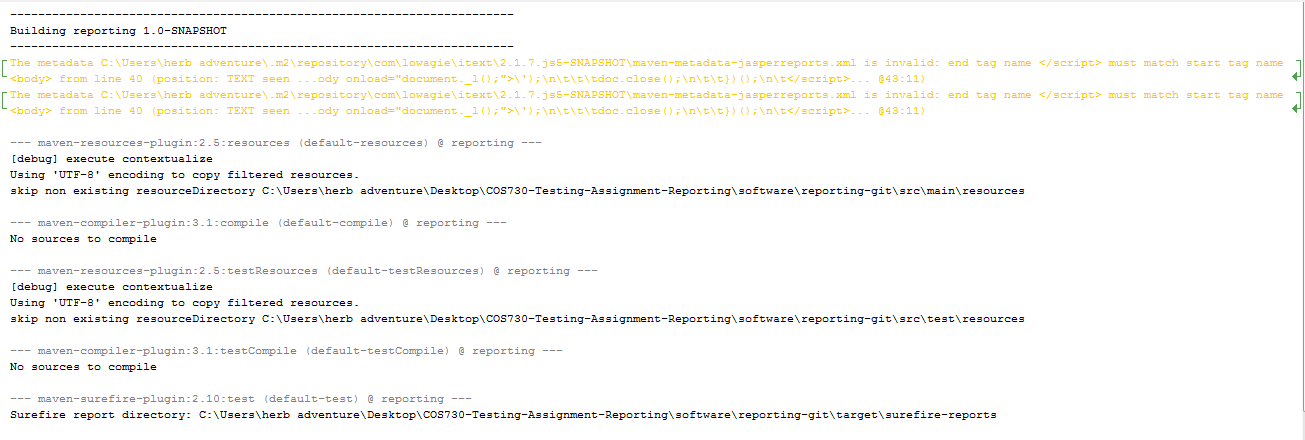
\includegraphics[scale=0.6]{mavenBuild1.PNG}
\end{figure} 
\begin{figure}[h!]
  \caption{Their tests}
	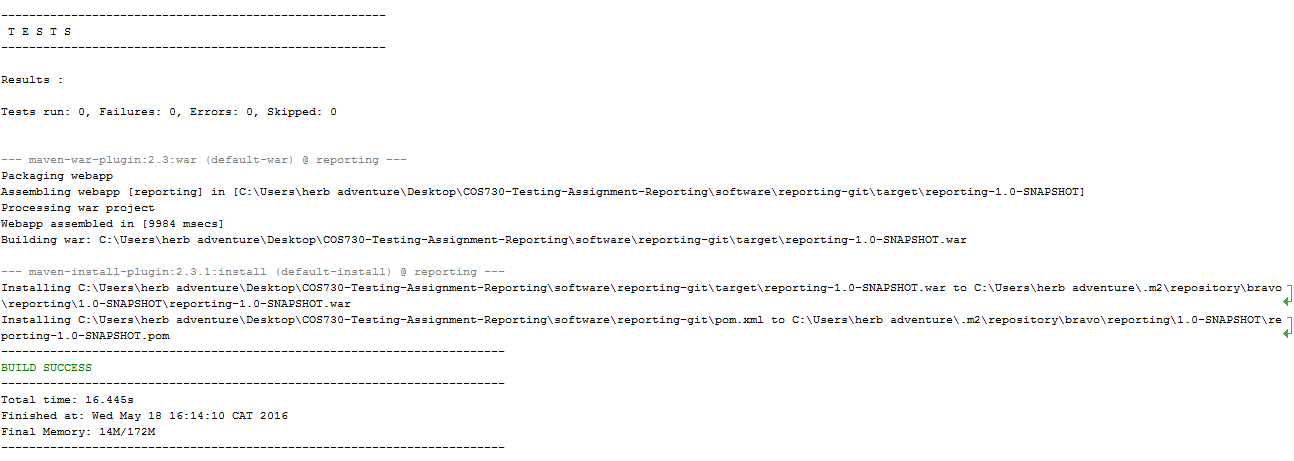
\includegraphics[scale=0.6]{mavenBuild2.PNG}
\end{figure} \\ \\
\item Use of Jasper Reports - Jasper Reports has not been used in the code and thus no reports are generated. There is no provision in the code for a framework such as Jasper Reports. 
\item Use of contracts and mock objects - The contracts specified in the Requirements Specification document have not been adhered to or implemented in the module. More specifically the two main services getAccreditationUnitsReport and getProgressReport and their functionality has not been implemented. In terms of mocking, no mocks have been used in the implementation and no mocking framework such as Mockito has been used in the unit tests provided either.
\item Deployable into application server -The code was not deployed on a server but it would not be ideal to deploy it on a server as a report cannot be generated and hence the functionality is not complete or correct.  
\end{enumerate}

\section{Rationale for Decisions}
Specify the issues that were considered for any decisions and the reason(s) for the selection of the
conclusion(s).

\section{Conclusions and Recommendations}
\label{sec:conclusions}
Specify an overall evaluation of each test item, including its limitations. This evaluation will be based
on the test results and on the item level pass/fail criteria. An estimate of failure risk may be included.
Recommend its status relative to availability for production use, and under what circumstances (e.g.,
immediately, with a specified subset of anomalies resolved, or never). This may include identification
of anomaly clusters in functionality and/or anomaly root cause analysis.
